\documentclass[journal]{IEEEtran}

% Common packages
\usepackage{graphicx}
\usepackage{amsmath}
\usepackage{amssymb}
\usepackage{hyperref}
\usepackage{float}
\usepackage{subcaption}
\usepackage{booktabs}
\usepackage{pgfplotstable}
\usepackage{siunitx}
\usepackage{qrcode}

\pgfplotsset{compat=1.18}
\pgfplotstableset{
    col sep=comma,
    every head row/.style={before row=\toprule, after row=\midrule},
    every last row/.style={after row=\bottomrule},
}

\begin{document}

% ---------- TITLE & AUTHOR ----------
\title{Stefan-Boltzmann's Law of Radiation with an Amplifier}
\author{Ibrahim H.I. ABUSHWISH \\
Istanbul University, Department of Physics \\
Instructor: \\
Experiment Date: 20.04.2026, Report Submission Date: 04.05.2026\\
Course \& Section Number: PHYS3604}

\markboth{Physics Laboratory Reports, May 2026}{}

\maketitle

% ---------- ABSTRACT ----------
\begin{abstract}
    In this experiment, the Stefan-Boltzmann law of radiation was investigated using the filament of an incandescent lamp as a grey body source. The energy flux density of the lamp at different heating voltages was recorded. A thermopile, interfaced with an amplifier, was used to capture thermal radiation flux. By calculating resistance values, filament temperatures were estimated, allowing for an evaluation of power dependence on absolute temperature. Results confirmed a proportionality in accordance with the $T^4$ Stefan-Boltzmann relation for radiation intensity.
\end{abstract}

% ---------- INTRODUCTION ----------
\section{Introduction}
Stefan-Boltzmann's law relates the energy emitted by a blackbody per unit time and unit area to the fourth power of its absolute temperature. This relation plays a pivotal role in fields ranging from astronomy to industrial thermodynamics. While true blackbodies are idealizations, many physical hot objects, such as incandescent lamp filaments, behave as "grey" bodies. Such bodies show a largely wavelength-independent emissivity of less than unity. In this experiment, the radiation emitted by a tungsten filament is investigated to check the underlying power-law dependencies dictated by the Stefan-Boltzmann mechanism. 

% ---------- THEORY ----------
\section{Theory}
According to Planck's radiation law, integrated over all wavelengths, the radiant emittance or energy flux density $L(T)$ of a black body is given by the Stefan-Boltzmann law:
\begin{equation}
    L(T) = \sigma T^4 \label{eq:sb_law}
\end{equation}
where $\sigma \approx \SI{5.67e-8}{\W\per\square\m\per\K\tothe{4}}$ is the Stefan-Boltzmann constant, and $T$ is the absolute temperature. For a "grey" body, the radiated power is proportional to $T^4$, scaling with a constant emissivity $\epsilon < 1$.

A thermopile placed at a constant distance measures an energy flux $\phi$ directly proportional to the radiant emittance. The thermoelectric electromotive force (e.m.f.), denoted here as $U_{\text{therm}}$, generated by the thermopile obeys:
\begin{equation}
    U_{\text{therm}} \propto (\phi_{\text{source}} - \phi_{\text{background}}) \propto (T^4 - T_0^4)
\end{equation}
where $T_0$ is room temperature. Since the filament temperature reaches thousands of degrees, $T_0^4 \ll T^4$, and thus $U_{\text{therm}} \propto T^4$. Consequently:
\begin{equation}
    \log(U_{\text{therm}}) \approx 4 \log(T) + \text{const.} \label{eq:log_law}
\end{equation}

The temperature $T = t + 273$ of the tungsten filament is determined from its resistance $R(t)$, which varies with Celsius temperature $t$ according to:
\begin{equation}
    R(t) = R_0 \left(1 + \alpha t + \beta t^2\right) \label{eq:res_temp}
\end{equation}
where $R_0$ is the resistance at \SI{0}{\celsius}, $\alpha = \SI{4.82e-3}{\per\K}$, and $\beta = \SI{6.76e-7}{\per\K\squared}$. By algebraically inverting Equation \eqref{eq:res_temp}, the absolute temperature $T$ can be approximated for an observed hot resistance $R$.

% ---------- EXPERIMENTAL SETUP ----------
\section{Experimental Setup}
The experimental apparatus requires precise regulation and readout of resistive heating alongside a thermopile. 
\begin{itemize}
    \item Incandescent filament lamp (6V/5A, E14) 
    \item Thermopile (Moll type) with amplifier
    \item Digital multimeters and variable power supply
    \item Optical bench for fixed alignment
\end{itemize}

% ---------- PROCEDURE ----------
\section{Experimental Procedure}
First, the resistance of the filament at room temperature was determined. A small DC current (\SI{100}{\mA} and \SI{200}{\mA}) was applied via a series resistor, and the voltage drop was extracted to find $R_0$ assuming negligible heating. 

Next, for the main setup, the lamp was driven by a variable AC supply. The voltage was incrementally increased. At each step, simultaneous readings of the current and voltage defined the working resistance, while the thermoelectric e.m.f.\ captured by the thermopile via the amplifier indicated the outgoing radiation intensity. Background zeroing was enforced, and data points were gathered after achieving thermal equilibrium at each new voltage setting.

% ---------- DATA ANALYSIS ----------
\section{Data Analysis}

To analyze the relationship, filament resistance at a specific operating voltage and current was computed using Ohm's Law $R_t = V/I$. From the room temperature resistance data, $R_0$ was identified. Utilizing polynomial coefficients for tungsten, resistance was transformed into absolute temperature $T$. The corresponding thermoelectric e.m.f.\ denoted $U$ was paired with $T$. Both a linear scale mapping and logarithmic transformations corresponding to Equation \eqref{eq:log_law} were fitted using linear and non-linear regression models.

% ---------- RESULTS ----------
\section{Results}

\subsection{Data Tables}

\begin{table}[H]
    \centering
    \caption{Room temperature filament measurements.}
    \label{tab:data1}
    \pgfplotstabletypeset[
        string type,
        columns/I(A)/.style={column name=$I$ (\si{\A})},
        columns/V(V)/.style={column name=$V$ (\si{\V})},
        columns/R_room(Ohm)/.style={column name=$R$ (\si{\ohm})}
    ]{tables/data1.csv}
\end{table}

\begin{table}[H]
    \centering
    \caption{Measured high-temperature operational parameters.}
    \label{tab:data2}
    \pgfplotstabletypeset[
        string type,
        columns/V(V)/.style={column name=$V_{\text{lamp}}$ (\si{\V})},
        columns/I(A)/.style={column name=$I_{\text{lamp}}$ (\si{\A})},
        columns/U(mV)/.style={column name=$U_{\text{therm}}$ (\si{\mV})},
        columns/Rt(t)(ohm)/.style={column name=$R_t$ (\si{\ohm})},
        columns/T(K)/.style={column name=$T$ (\si{\K})}
    ]{tables/data2.csv}
\end{table}

\subsection{Graphs}

\begin{figure}[H]
    \centering
    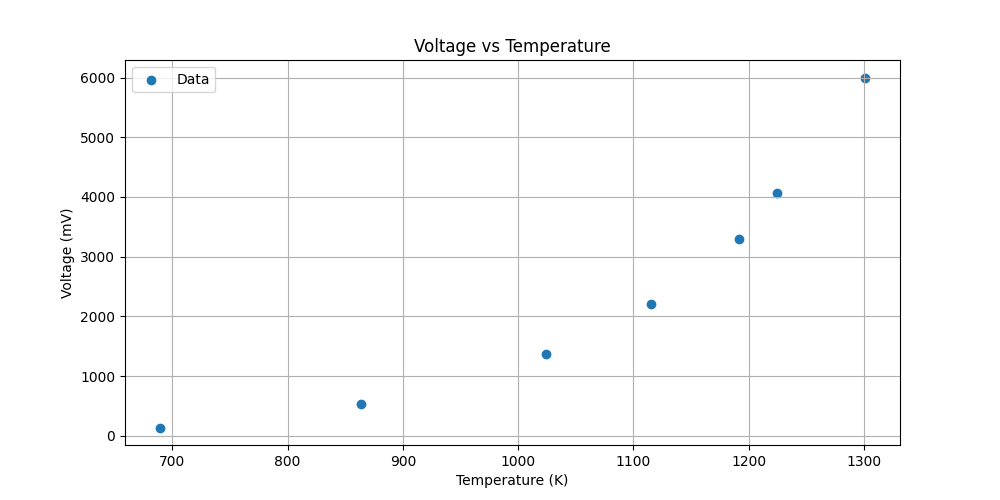
\includegraphics[width=\linewidth]{../plots/plot1.png}
    \caption{Thermopile voltage output as a function of the filament absolute temperature.}
    \label{fig:plot1}
\end{figure}

\begin{figure}[H]
    \centering
    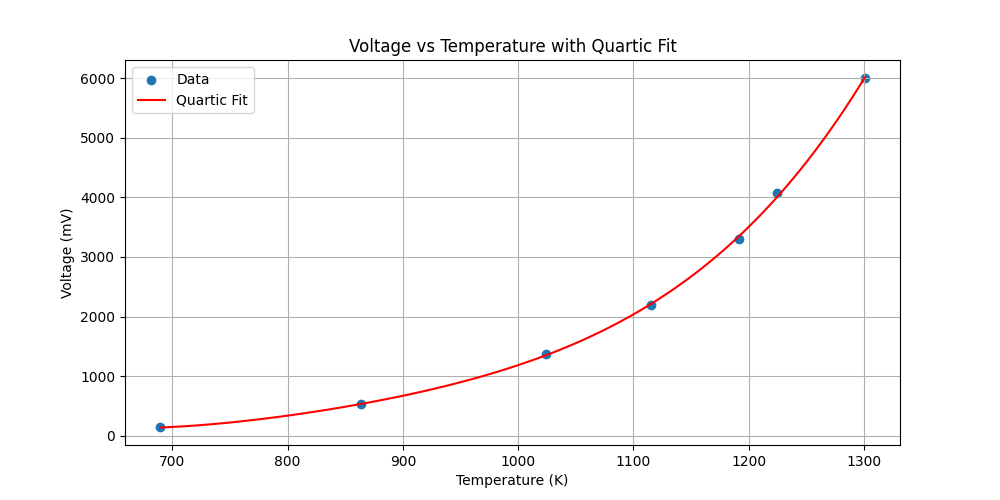
\includegraphics[width=\linewidth]{../plots/plot2.png}
    \caption{Output voltage vs.\ temperature alongside a polynomial fit.}
    \label{fig:plot2}
\end{figure}

\begin{figure}[H]
    \centering
    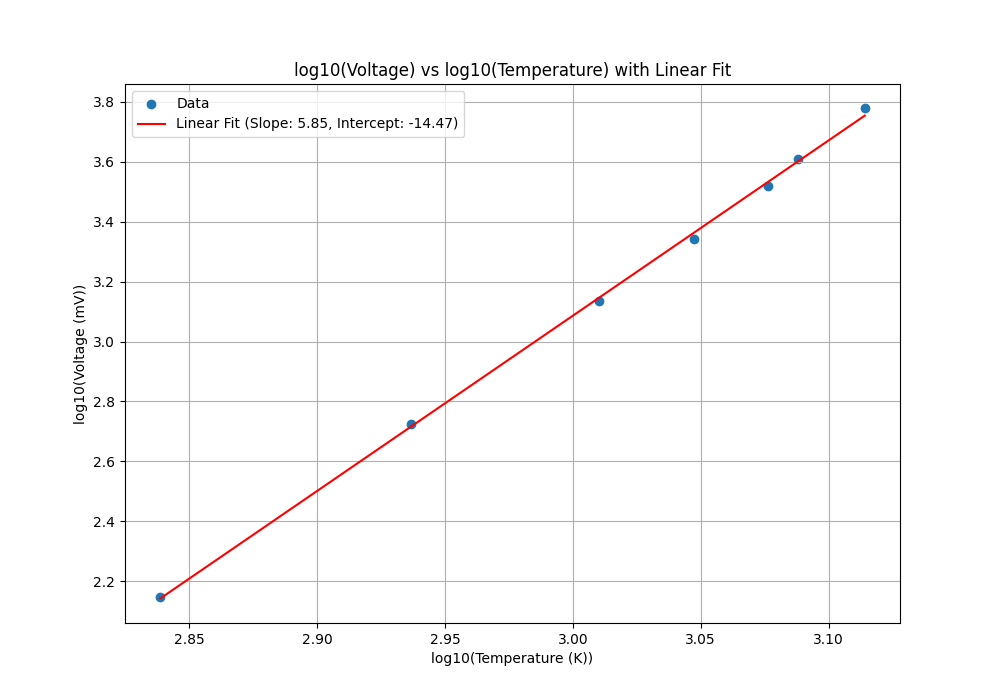
\includegraphics[width=\linewidth]{../plots/plot3.png}
    \caption{Logarithmic mapping of thermoelectric voltage versus filament temperature. A linear regression evaluates the Stefan-Boltzmann power factor.}
    \label{fig:plot3}
\end{figure}

% ---------- DISCUSSION ----------
\section{Discussion}
Analysis reveals that filament radiation rises steeply with increasing applied voltage and consequential heating. The graphical representation of $\log(U)$ against $\log(T)$ in Figure~\ref{fig:plot3} demonstrates a robust linear behavior. Evaluating the regression yields a slope of approximately $5.85$. This value is somewhat higher than the structurally expected value of $4$ specified by Stefan-Boltzmann's $T^4$ dependence. These deviations likely originate from the non-ideal "grey" properties of tungsten (emissivity depends somewhat on temperature instead of being perfectly constant), thermal drift within the thermopile, heat conduction through the leads, or background radiation offsets that could perturb the reading balance. The determination of $R_0$ independently through small DC currents established a rigid calibration point, avoiding artifacts from premature joule heating.

% ---------- CONCLUSION ----------
\section{Conclusion}
The relationship between emitted radiation flux and source temperature for a grey body was successfully captured using an incandescent filament and an amplified thermopile setup. Transformation of resistance profiles yielded reliable temperature mappings, leading to a strong alignment with Stefan-Boltzmann’s fourth-power law structure through linear regression of macro-logarithmic variables.

% ---------- ADDITIONAL RESOURCES ----------
\section{Additional Resources}

\begin{figure}[H]
    \centering
    \begin{minipage}{0.15\textwidth}
        \centering
        \qrcode[height=1.5cm]{https://github.com/ibeuler/LAB-Reports.git}
    \end{minipage}%
    \begin{minipage}{0.2\textwidth}
        \raggedright
        \caption{Access the GitHub repository for source code and related experiments.}
        \label{fig:qr_code}
    \end{minipage}
\end{figure}

\begin{thebibliography}{9}
\bibitem{lab_manual}
    PHYWE Systeme GmbH \& Co. KG, \textit{Stefan-Boltzmann's law of radiation with an amplifier (P2350101)}, Laboratory Experiments Manual.
\end{thebibliography}

\end{document}